% !TeX root = ..//diffgeo_main.tex
Im Folgenden werden nun einige Beispiele für Vektorbündel angeben.
\subsection{Direkte Summe (Whitney-Summe)}
Es seien zwei Vektorbündel gegeben:
\begin{align}
\pi : E &\to \mfk \\
\pi ' : E' & \to \mfk '
\end{align}
mit $\rang$ $k$ bzw. $k'$. 
Dann existiert $(U_\alpha)_{\alpha \in A}$ eine offene Überdeckung, sodass für alle $\alpha \in A$ und alle $p \in U_\alpha$ folgendes gilt:
\begin{align}
&\phi_{\alpha, p}: \R^k \to E_p, \quad g_{\alpha, \beta}: U_\alpha \cap U_\beta \to \mathrm{Gl}(k, \R)\\
&\phi_{\alpha, p}': \R^{k'} \to E_{p}', \quad g_{\alpha, \beta}': U_\alpha \cap U_\beta \to \mathrm{Gl}(k', \R)
\end{align}  
Wir definieren:
\begin{align}
&\mathcal{E}_p := E_p \oplus E_{p}\\
&\mathcal{E} = \bigcup_{p \in \mfk} \mathcal{E}_p
\end{align}
\begin{align}
&\Phi_{\alpha, p}: \R^k \oplus \R^{k'} \to E_P \oplus E_{p}'\\
&(v, w) \mapsto (\phi_{\alpha \ p} (v), \phi_{\alpha \ p}' (w))
\end{align}
\begin{align}
&G_{\alpha \beta}: U_\alpha \cap U_\beta \to \mathrm{Gl}(k + k', \R)\\
&p \mapsto \begin{pmatrix}
g_{\alpha \beta}(p)  & 0 \\ 
0  & g_{\alpha \beta}'(p)
\end{pmatrix} 
\end{align}
$\mathcal{E}$ ist nun ein Vektorbündel. 
Wir nennen $\mathcal{E}$ die Whitney-Summe von $E$ und $E'$ und schreiben:
\begin{align}
\mathcal{E} = E \oplus E'.
\end{align} 

\subsection{Tensorbündel}
Es seien $E'$ und $E''$ Vektorbündel über $\mfk$ und $(U_\alpha)$ sei wie oben definiert.
\begin{align}
(E' \oplus E'')_p &:= E_{p}'\oplus E_{p}''\\
\phi_{\alpha \ p} : \R^{k'} \times \R^{k''} &\to E_{p}' \oplus E_{p}''\\
(v, w) &\mapsto \phi_{\alpha \ p}'(v) \oplus \phi_{\alpha \ p}'' (w)
\end{align}
Wir erhalten zusammen die Folgende Übergangsmatrix:
\begin{align}
g_{\alpha \beta} = g_{\alpha \beta}'(p) \oplus g_{\alpha \beta}''(p)
\end{align}
Diese Abbildung ist glatt und somit ergibt sich somit ein neues Vektorbündel.

\subsection{Homomorphismenbündel}
Es seien die Daten wie eben schon gegeben.
Das Homomorphismenbündel
\begin{align}
\mathrm{Hom}_p := \mathrm{Hom}(E_{p}', E_{p}'')
\end{align}
ist wie folgt gegeben:
\begin{align}
\phi_{\alpha \ p} : \mathrm{Hom}(\R^{k'}, \R^{k''}) &\to \mathrm{Hom}(E_{p}', E_{p}'')\\
f &\mapsto \phi_{\alpha \ p} \circ f \circ (\phi_{\alpha \ p}')^{-1}
\end{align}

\subsection{Duales Bündel}
Sei ein Vektorbündel $(\pi, E, \mfk)$ gegeben. 
Wir wollen nun das sogenannte duale Vektorbündel konstruieren.
Hierbei führen wir folgende Notation ein $E^* = \mathrm{Hom}(E, \R)$.
Hierbei ist $\R$ das triviale Vektorbündel vom Rang $1$.
Ein wichtiges Beispiel ist hierbei das Kotangentialbündel $T^{*}\mfk = \mathrm{Hom}(T\mfk , \R)$.
$T^{*}_{p}\mfk$ heißt der Kotangentialraum.\\
Sei $f: \mfk \to \R$ eine glatte Abbildung.
\begin{align}
\dd f \big\vert_p : T_p \mfk \to T_{f(p)}\R \cong \R
\end{align}
Es gilt $\dd f\big\vert_p \in T_p^* \mfk \subset T^* \mfk$.
Sei $x: U \to x(U)$ eine Karte 
\begin{align}
\dd x \big\vert_p : T_p \mfk \to \rn
\end{align}
Die so definierten Differentiale $\{ \dd x^1 \big\vert_p, \dots , \dd x^n \big\vert_p \}$ bilden eine Basis für $T_p^* \mfk$.
\begin{itemize}
\item $\dd x^i \big\vert_p$ heißen Kotangentialvektoren
\item $\pdv{x^i} \big\vert_p$ heißen Tangentialvektoren
\end{itemize}
Seien $(x, U)$ und $(y, U')$ zwei Karten um p.
\begin{align}
\pdv{x^i}\big\vert_p &= \sum_j a^j_i \pdv{y^j} \big\vert_p, \quad a^j_i = \pdv{y^j}{x^i} \\
\dd x^k &= \sum b^k_l \dd y^l \big\vert_p = \sum \pdv{x^k}{y^l} \dd y^l \big\vert_p
\end{align}

\subsection{Alternierendes Vektorbündel}
Das Alternierende Vektorbündel
\begin{align}
\wedge^m(E', E'')_p &:= \wedge^m(E_{p}', E_{p}'')\\
&= \{ f: \underbrace{E_{p}' \times \dots \times E_{p}'}_{n-\mathrm{mal}} \to E_{p}'' \}
\end{align}
Wobei $f$ multilinear und alternierend ist. 
\begin{align}
&\phi_{\alpha \ p}: \wedge^n (\R^{k'}, \R^{k''}) \to \wedge^n (E_{p}', E_{p}'')\\
&f \mapsto ((v_1, \dots, v_n) \mapsto \phi_{\alpha p}''( f(\phi_{\alpha p})^{-1} (v_1), \dots f(\phi_{\alpha p})^{-1} (v_n)) )
\end{align}
Es bleibt zu zeigen, dass $g_{\alpha \beta}$ glatt ist.\\
Es gilt 
\begin{align}
\wedge^1 (E', E'') &= \mathrm{Hom}(E', E'')\\
\wedge^1 (T\mfk, \R) &= T^{*}\mfk
\end{align}

\begin{defs}[Bündel-Abbildung]
Seien $(\pi, E, \mfk)$ und $(\pi, E', \mfk')$ Vektorbündel.
Ein paar $(f, L)$ von glatten Abbildungen $f: \mfk \to \mfk'$ und $L: E \to E'$ heißt Bündelabbildung falls:
\begin{itemize}
\item $\pi' \circ L = f \circ \pi$
\item $L\big\vert_{E_p}$ ist $\R$-linear
\end{itemize}


\begin{align}
\begin{xy}
  \xymatrix@=0.25\linewidth{
      E \ar[r]^L \ar[d]_\pi    &   E' \ar[d]^{\pi '}  \\
      \mfk \ar[r]_f             &   \mfk'   
  }
\end{xy}
\end{align}
\end{defs}

\begin{bsp}
Seien $\mfk$,$\mfk'$ glatte Mannigfaltigkeiten und $f:\mfk \to \mfk'$ glatt.
Dann ist $(f, \dd f)$ eine Bündel-Abbildung von $T\mfk$ nach $T\mfk'$.
\end{bsp}

\begin{defs}[Unterbündel]
Sei $(\pi, E, \mfk)$ ein Vektorbündel mit Rang $k$.
Eine Untermannigfaltigkeit $E' \subset E$ ist ein Unterbündel vom Rang $k'$ falls
\begin{align}
\pi \big\vert_{E'}: E' \to \mfk,
\end{align}
Ein Vektorbündel ist.
\end{defs}

\begin{bsp}[Unterbündel] \leavevmode
\begin{enumerate}
\item $S^n \subset \R^{n+1}$
\begin{align}
TS^m \cong \{ (p,x)\in S^n \times \R^{n+1} \vert x \perp p \} \subset \underbrace{S^n \times \R^{n+1}}_{\mathrm{triviales} \ \mathrm{Bündel}}
\end{align}
ist ein Unterbündel
\item $\R \mathbb{P}^n$ mit dem tautologischen Bündel 
\begin{align}
\{ (l, x) \in \R \mathbb{P}^n \times \R^{n+1} \vert x \in l \} \subset \R\mathbb{P}^n \times \R^{n+1}
\end{align}
ist ein Unterbündel.
\end{enumerate}
\end{bsp}
\begin{defs}[Schnitte von Vektorbündeln]
Sei $(\pi, E, \mfk)$ ein Vektorbündel.
Eine glatte Abbildung $s:\mfk \to E$ heißt Schnitt von $E$, falls $\pi \circ s = \id\big\vert_{\mfk}$.
Wir bezeichnen die Schnitte von $E$ mit $\Gamma (E)$.
Sei $U \subset \mfk$. 
Ein Schnitt von $E$ über $U$ ist eine Abbildung $s : U \to E$ mit $\pi \circ s = \id_U$.
\begin{figure}[H]
\centering
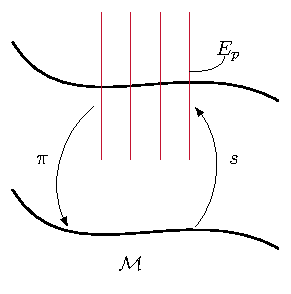
\includegraphics[width=0.4\linewidth]{figures/tikz/section_fiber_bundle.pdf}
\label{img:bspvektorfeld}
\end{figure} 
\end{defs}
\begin{bsp}[Schnitte] \leavevmode
\begin{itemize}
\item Nullschnitt
\begin{align}
&s : \mfk \to E \\
&p \mapsto 0 \in E_p
\end{align}
\item Schnitte von $T\mfk$ heißen Vektorfelder.
Wir bezeichnen die Vektorfelder $V: \mfk \to T\mfk$ mit $\mathfrak{X}(\mfk)$.

\begin{figure}[h]
\centering
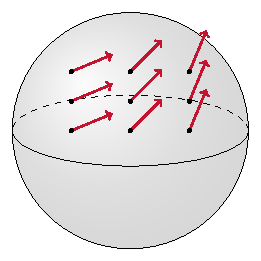
\includegraphics[width=0.4\linewidth]{figures/tikz/vectorfield_on_manifold.pdf}
\caption{Beispiel für ein Vektorfeld}
\label{img:bspvektorfeld}
\end{figure} 

\end{itemize}
\end{bsp}


\begin{satz}
\label{satz:SchnitteModul}
Der Raum der Schnitte $\Gamma (E)$ ist ein Modul über $\mathcal{F}(\mfk)$.
\end{satz}

\begin{bew}[Satz \ref{satz:SchnitteModul}]
Seien $s_1, s_2 \in \Gamma (E)$, so ist $s_1 + s_2 \in \Gamma (E)$
\begin{align}
(s_1 + s_2)(p) := s_1 (p) p s_2 (p)
\end{align}
Sei $\phi \in \mathcal{F}(\mfk), s\in \Gamma(E)$, so ist $\phi \circ s \in \Gamma (E)$
\begin{align}
(\phi \circ s) (p) := \phi (p) s(p).
\end{align}
\end{bew}

\begin{lem}
Sei $(\pi, E, \mfk)$ ein Vektorbündel und $p \in \mfk$.
Dann gilt für alle $x \in E_p$ existiert ein Schnitt $s \in \Gamma (E)$, so dass $s(p)=x$
\end{lem}
\begin{bew}
Wähle eine lokale Trivialisierung von $E$ auf $W \ni p$
\begin{align}
\phi: W \times \R^k \to \pi^{-1}(W) = E\big\vert_W
\end{align}
und eine glatte Funktion $\varphi \in \mathcal{F}(\mfk)$ mit $\varphi(p)=1$ und $\supp(\varphi) \subset W$.
Sei $\xi \in \R^k$, so dass $\phi (p, \xi)=x$.
Definiere:
\begin{align}
s(q) = \left\{
\begin{array}{ll}
\phi(q, \varphi(q)\xi) & q\in W \\
0_q & q \not\in W \\
\end{array}
\right.
\end{align}
$s$ ist glatt, da folgendes gilt:
\begin{itemize}
\item $s$ ist glatt auf $W$
\item $s$ ist $0$ auf einer Umgebung von $\mfk \setminus W$
\end{itemize}
\begin{align}
s(p) = ( \varphi(p), \varphi(p) \xi ) = \varphi (p \xi) = x
\end{align}
\end{bew}

\begin{defs}[Lokaler Rahmen]
Sei $(\pi, E, \mfk)$ ein Vektorbündel vom Rang $k$ und $U \subset \mfk$.
Ein Rahmen von $E$ über $U$ ist ein $k$-Tupel.
$(s_1, \dots, s_k)$ von glatten Schnitten über $U$ (das heißt $s_i \in \Gamma_i (E)$), so dass für alle $p \in U$
$s_1 (p), \dots, s_k (p)$ eine Basis von $E_p$ bilden.
\end{defs}